%!TEX root = ../Thesis.tex
\section{Projektplanung}
\fancyhead[R]{Projektplanung}
\label{instal}

\subsection{Beschreibung des Funktionsumfangs (Florian Rath)}
%%%%%%%%%
%Florian
%%%%%%%%%

Im Rahmen des Projektes „TEN-Manager“ müssen einige Funktionen umgesetzt werden. Die App soll die Verwaltung von Aufgaben (Todos), Ereignissen (Events) und Notizen (Notes) ermöglichen, diese Einträge werden als TENs bezeichnet.

Dem Benutzer sollen für alle TENs die Grundfunktionen Erfassung, Veränderung, Löschung und Betrachtung zur Verfügung stehen. Außerdem soll es dem Benutzer möglich sein die Ansicht einzelner TENs aufzurufen und dort die Eingabefunktion benutzen zu können. Die Funktionen sollen eine einfache und intuitive Bedienbarkeit aufweisen. Die Funktionalität soll durch eine minimale Menge von Interaktionen bestechen und die ganze App soll durch eine ansprechende und übersichtliche Gestaltung der Benutzeroberfläche visualisiert werden. Die App besteht aus vier Hauptansichten, die der Todos, Events und Notes, jede dieser Ansichten, soll wenn sie erstellt wurde in einer kürzeren Version in einer allgemeinen Übersicht dargestellt werden. Mit Todos sind Aufgaben gemeint, die der Benutzer erledigen möchte oder muss, diese sollen einen Titel, eine Beschreibung, einen Zeitraum und die Todos enthalten. Der Fortschritt der Todos soll durch eine Prozentanzeige angezeigt werden. 
Durch die Events soll der Benutzer zu spezifizierten Zeitpunkten an Ereignisse erinnert werden. Dazu kann der Benutzer einen beschreibenden Text eingeben. Außerdem soll der Benutzer entscheiden können, an welchen Zeitpunkten eine Erinnerung erfolgen soll.

Die Notes ermöglichen es dem Benutzer Informationen zu speichern. Die Informationen können aus einer Notiz, Stichworten und Bildern bestehen. Die Daten der verschiedenen Ansichten sollen in einer Datenbank gespeichert werden, bzw. die Daten sollen dann auch wieder aus der Datenbank geladen werden können.

\newpage
\subsection{Projektablaufplan (Fabia Schmid)}
%%%%%%%%%
%Fabia
%%%%%%%%%

Als Projektleiterin wählte ich als Vorgehensmodell für die Entwicklung das erweiterte Wasserfallmodell fest. Dafür sprach die klare Struktur des Modelles und der geringe Managementaufwand. Zusätzlich war die Übersichtlichkeit, sowie die leichte Verständlichkeit ein klarer Vorteil. Außerdem sprach für das erweiterte Wasserfallmodell, dass es für kleine Projekte mit festgelegten Umfang ausgelegt und geeignet ist.

Auf diesem Vorgehensmodell basierte die Projektstrukturplanung, die Meilensteinplanung und die Zeitplanung, welche in einem GANTT-Diagramm visualisiert wurde.

\begin{figure}[H]
\centering
\begin{minipage}[t]{1\textwidth} % Breite, z.B. 1\textwidth		
\caption{Projektstrukturplan} % Überschrift
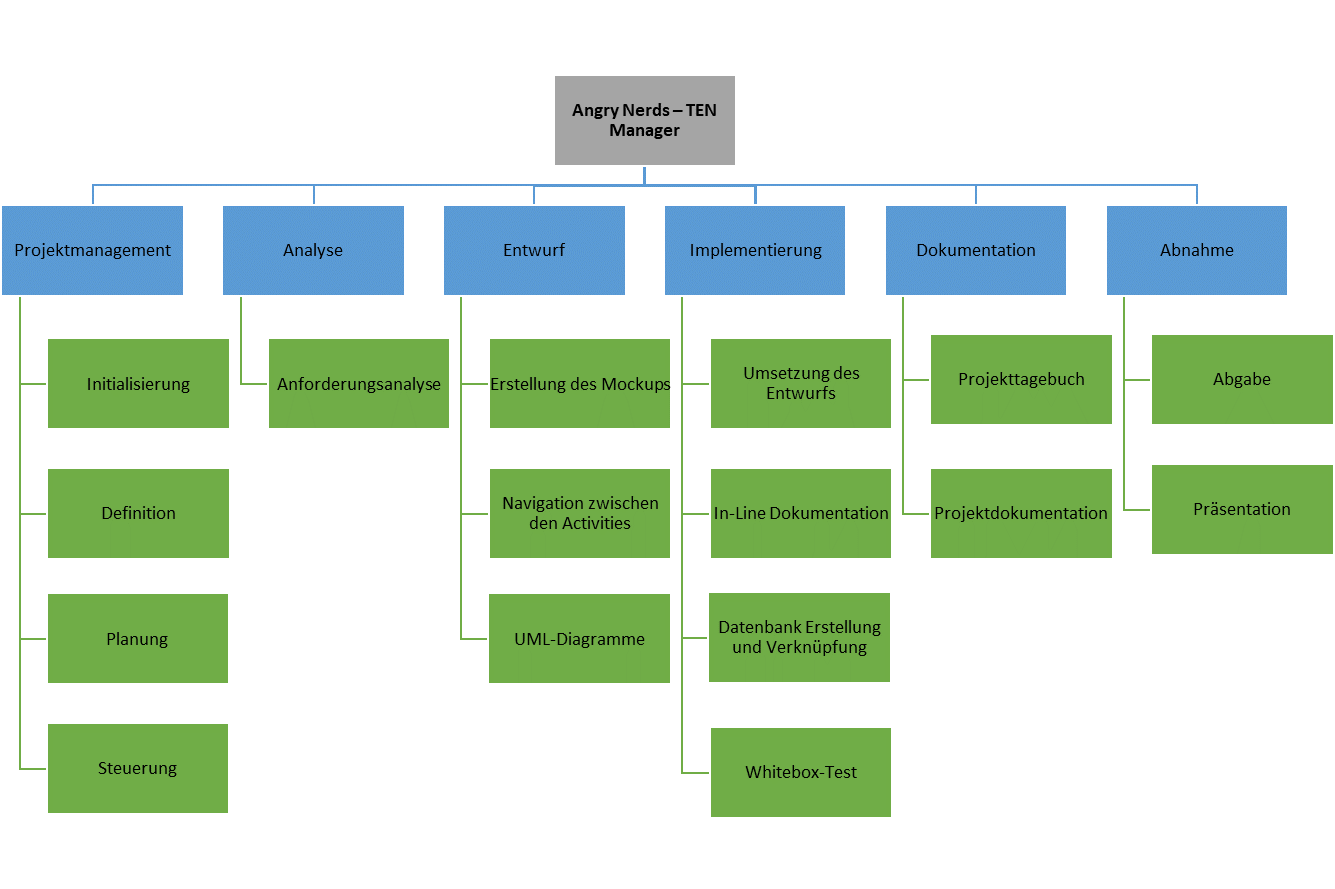
\includegraphics[width=13cm]{img/Projektstrukturplan}\\ % Pfad
\source{Erstellt von Fabia Schmid} % Quelle
\end{minipage}
\end{figure}

\begin{table}[H]
\caption{Meilensteinplan} % Überschrift
\begin{tabular}{|p{2cm}|p{9cm}|p{3cm}|}
\hline
{\textbf{ID}} & {\textbf{Meilenstein}} & {\textbf{Datum}} \\ \hline
1 & Kick-Off gehalten & 05.09.2018 \\ \hline
2 & Vorgehensmodell ausgewählt & 12.09.218 \\ \hline
3 & Datenbankmodel ausgewählt & 14.09.2018 \\ \hline 
4 & Activities verteilt & 20.09.2018 \\ \hline
5 & Mockup fertig & 20.09.2018 \\ \hline
6 & Activities und Layouts fertig & 01.12.2018 \\ \hline
7 & Activities getestet & 10.12.2018 \\ \hline
8 & Activities zusammengeführt & 20.12.2018 \\ \hline
9 & App getestet & 05.01.2019 \\ \hline
10 & Dokumentation fertig & 01.02.2019 \\ \hline
11 & Ausarbeitungsabgabe & 07.02.2019 \\ \hline
12  & Präsentation & 09.02.2019\\ \hline
\end{tabular}
\end{table}

\begin{figure}[H]
\centering
\begin{minipage}[t]{1\textwidth} % Breite, z.B. 1\textwidth		
\caption{GANTT-Diagramm} % Überschrift
\includegraphics[width=9cm]{img/GANTT}\\ % Pfad
\source{Erstellt von Fabia Schmid} % Quelle
\end{minipage}
\end{figure}

\newpage
\subsection{Planung der Software}
\subsubsection{Planung des Mock-Ups (Robin Menzel)}
%%%%%%%%%
%Robin
%%%%%%%%%
Das Mockup wurde von Beginn der Projektes an erstellt und ist das Ergebnis vieler Änderungen und Versionen. Während beim ersten Meeting zum Aussehen der App bereits Stilrichtung und Präferenzen der Gruppenmitglieder festgehalten wurden, entstand das erste Mock-Up erst einige Zeit später. Neben Handschriftlichen Zeichnungen zu Beginn des Designs, war das Programm Adobe Xd das ausgewählte Werkzeug für das Mock-Up. Adobe Xd war zu Beginn des Projektes erst in einer Beta Version verfügbar, welche für unsere Ansprüche jedoch ausreichte. Es ist ein vektorbasiertes Tool zum Entwerfen und Prototyping der User Experience für webbasierte und mobile Applikationen.

Das Design leitet sich von Googles Designsprache \textit{Material Design} ab, welche besonders durch die materialartigen, kartenähnlichen Flächen und das Flat Design charakterisiert wird. Außerdem ist das Layout und die Farbgestaltung angelehnt an verschieden Applikationen, wie z.B.
\begin{itemize}
\item Google Notizen
\item Google Kalender
\item Google Fotos
\item Wunderlist
\end{itemize}
Dies liegt vor allem daran, das in diesen Applikationen das Material Design sehr gut umgesetzt wurde. Aus Google Notizen wurde die Übersichtsseite und die charakteristische, schwebende Appbar übernommen. So sind auch unsere TENs in der Übersichtsseite als Fragmente dargestellt, in denen sich die wichtigsten Informationen schnell ablesen lassen. Die Detail- bzw. Bearbeitungsseiten der TENs wurde angelehnt an die Bearbeitungsseite des Google Kalenders. Hier wurden die Kategorien bzw. Einstellmöglichkeiten durch feine Linien visuell voneinander abgetrennt. Durch die eindeutigen Icons und dem auslassen von Beschriftungen wird der Bildschirm optimal genutzt. Auch Wunderlist schafft es in den Detailansichten von ToDos mit wenigen Hinweisen, ein minimalistische, aber ituitive und vorallem infomative Darstellung zu schaffen, von der wir uns inspiriert haben. Bei Google Fotos wurde die untere Navigationsleiste übernommen. So ist es in unserer App nun möglich mit einem Klick zwischen einer Übersicht über alle TENs, zu einer Übersicht über die unterschiedlichen Kategorien zu wechseln. Dies nutzt auf effektive Weise den Platz auf dem Tablet und bietet die Funktion an einer intuitiven Position an. Außerdem können wir so auf einen so genannten Navigation Drawer verzichten, da dieser die Applikation unnötig aufplustert und unsere Applikation kaum Funktionalitäten anbietet, die in diesem Drawer positioniert werden hätte können.

In Adobe Xd lassen sich nicht nur die Oberflächen Designen, sondern auch die User Experience abbilden. So lassen sich Flächen mit einander Verbinden, die nun durch einen Klick geöffnet werden können. Auf diese Art und Weise war es uns möglich Personen aus unserem Umkreis unsere App testen zu lassen. Das Feedback war ausschließlich Positiv. Da wir Elemente aus oft genutzten Apps übernommen haben, stellte die Bedienung unserer App für alle Tester kein Problem dar. Außerdem kam das Feedback, das unsere Oberfläche zur ersten Nutzung einlädt und nicht durch Überladung von Informationen abschreckt.

\begin{figure}[H]
\centering
\begin{minipage}[t]{1\textwidth} % Breite, z.B. 1\textwidth		
\caption{Mockups - Übersicht über alle TENs} % Überschrift
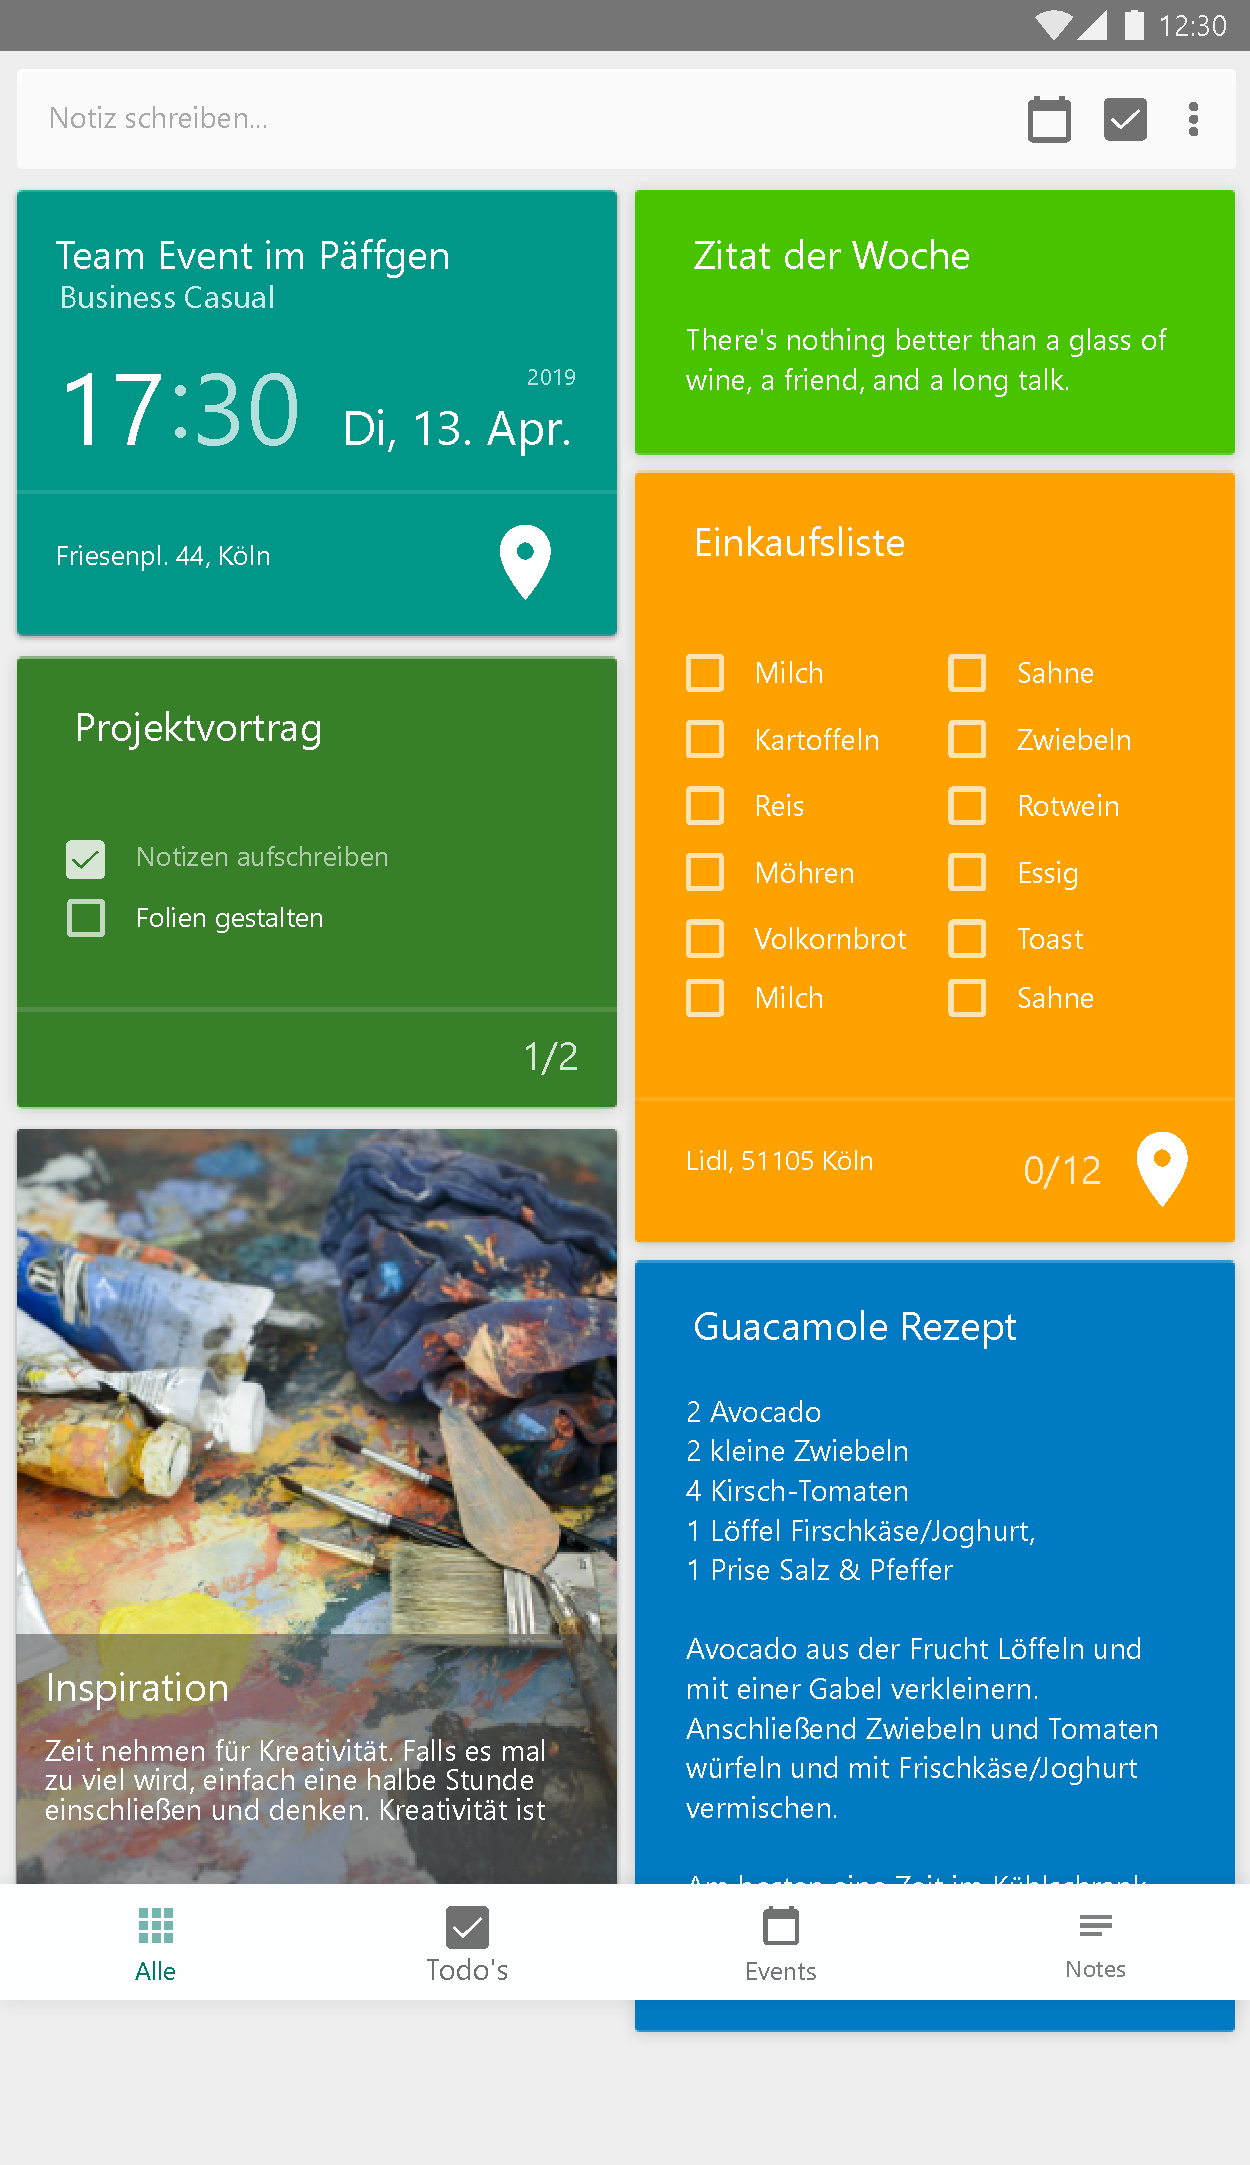
\includegraphics[height=20cm]{img/OverviewActivity}\\ % Pfad
\source{Erstellt von Robin Menzel} % Quelle
\end{minipage}
\end{figure}

\begin{figure}[H]
\centering
\begin{minipage}[t]{1\textwidth} % Breite, z.B. 1\textwidth		
\caption{Mockups - Übersicht über ein vorhandenes und ein neues Event} % Überschrift
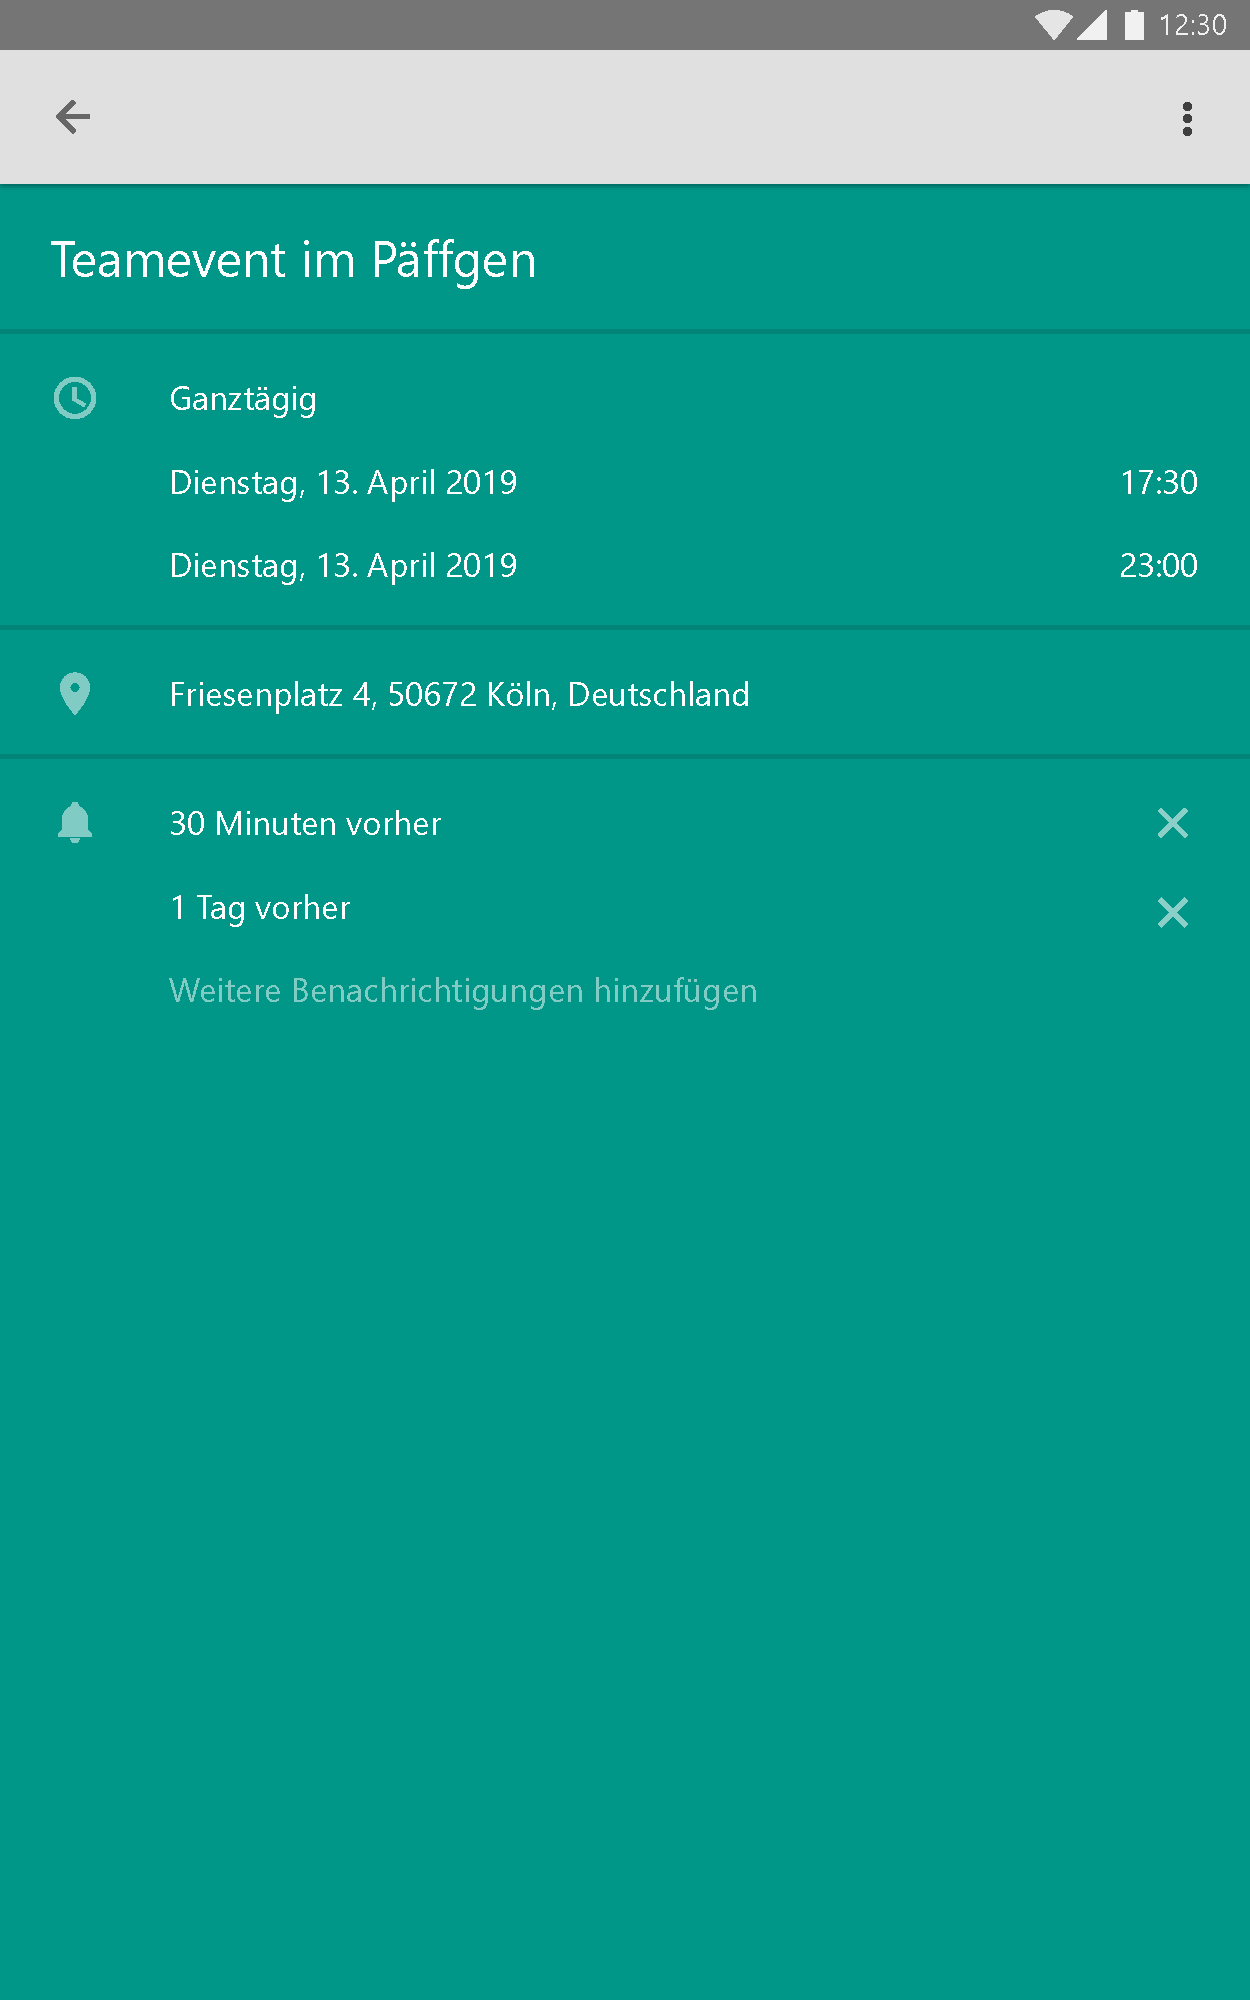
\includegraphics[width=7.25cm]{img/EventActivity} % Pfad
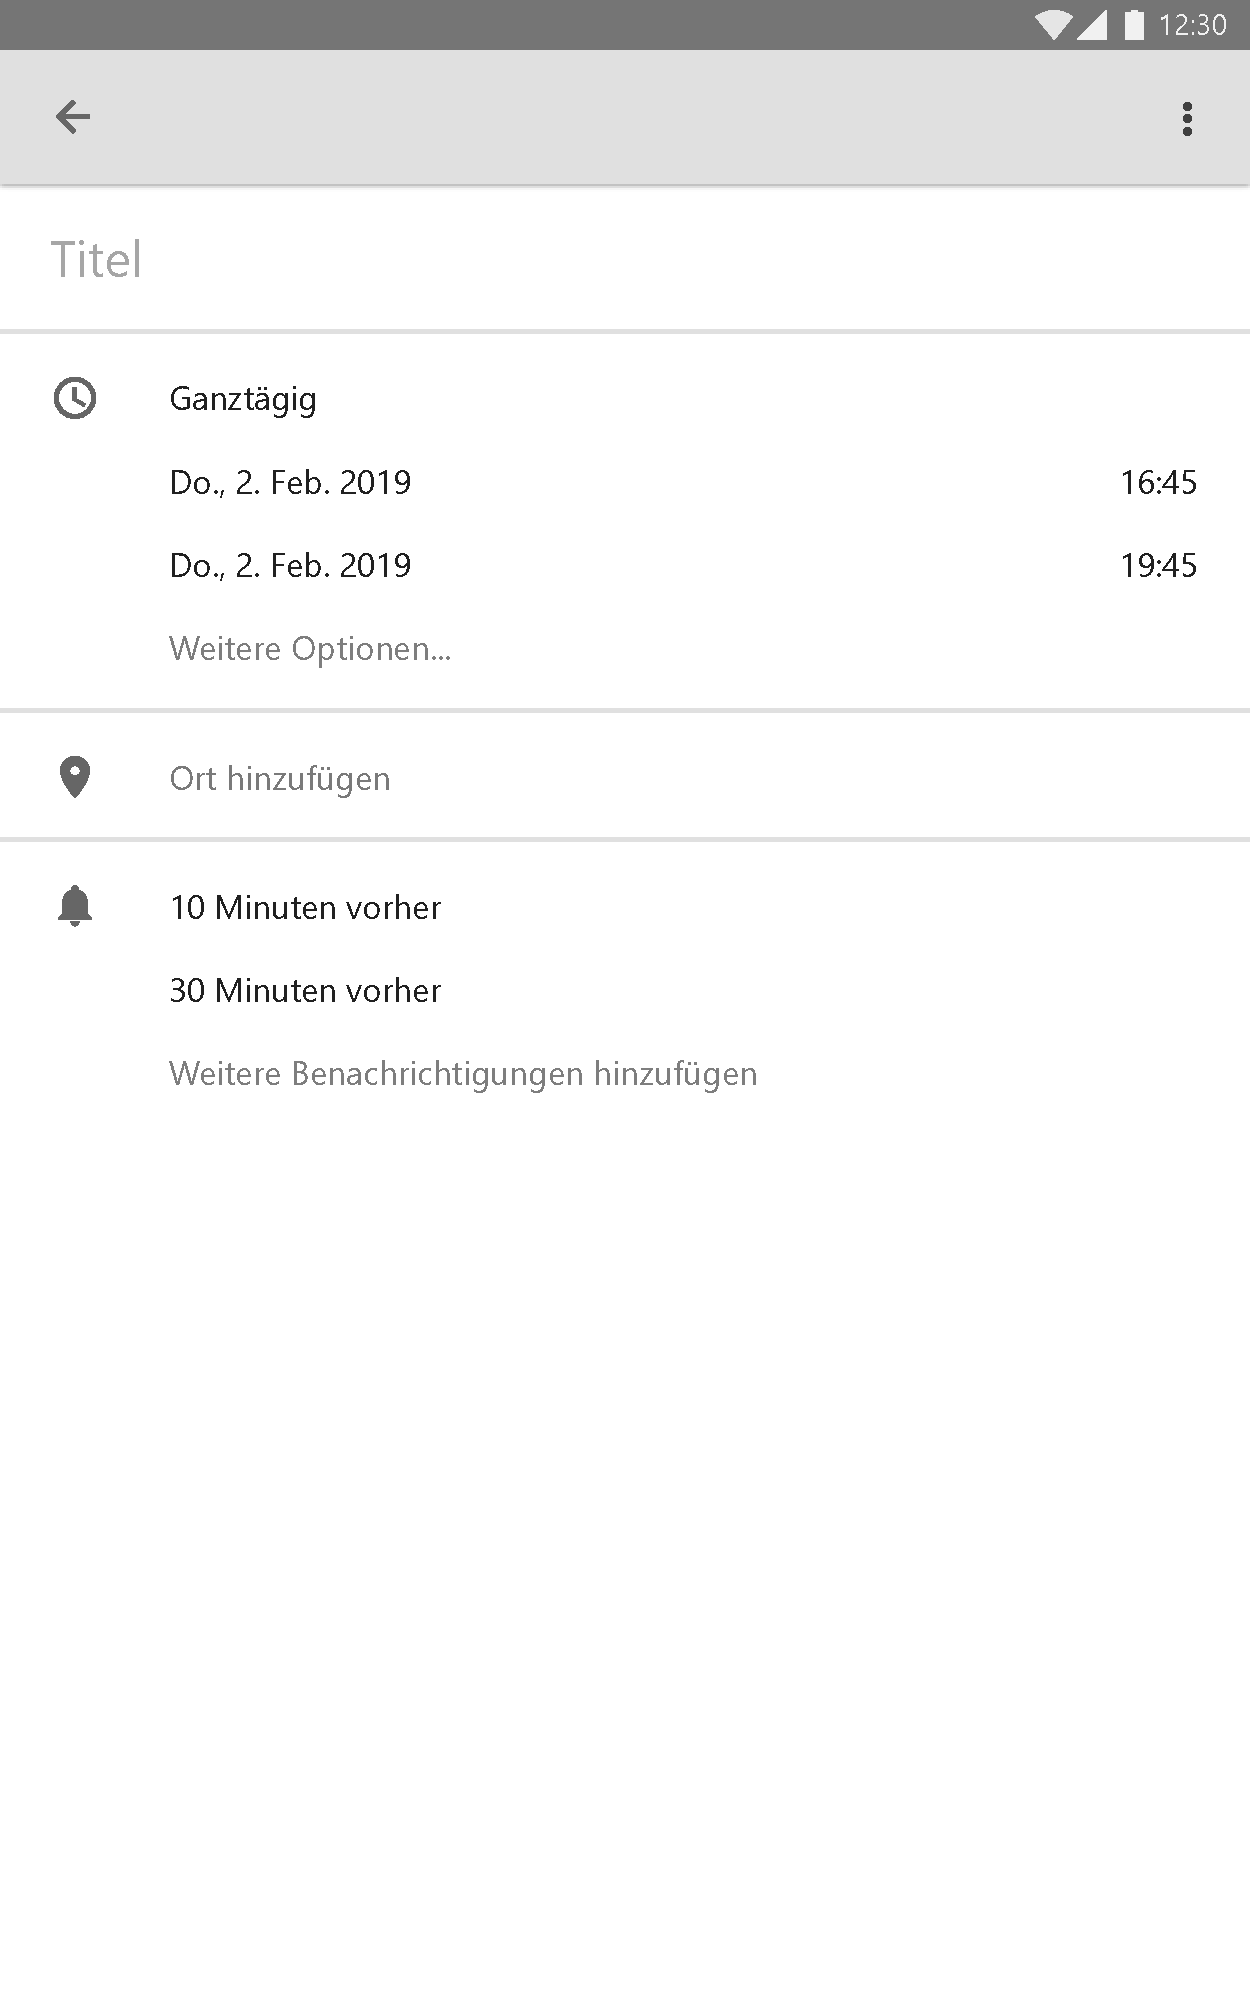
\includegraphics[width=7.25cm]{img/EventActivityNew}\\ % Pfad
\source{Erstellt von Robin Menzel} % Quelle
\end{minipage}
\end{figure}

\begin{figure}[H]
\centering
\begin{minipage}[t]{1\textwidth} % Breite, z.B. 1\textwidth		
\caption{Mockups - Übersicht über ein vorhandene, eine leere und eine Bild-Notiz} % Überschrift
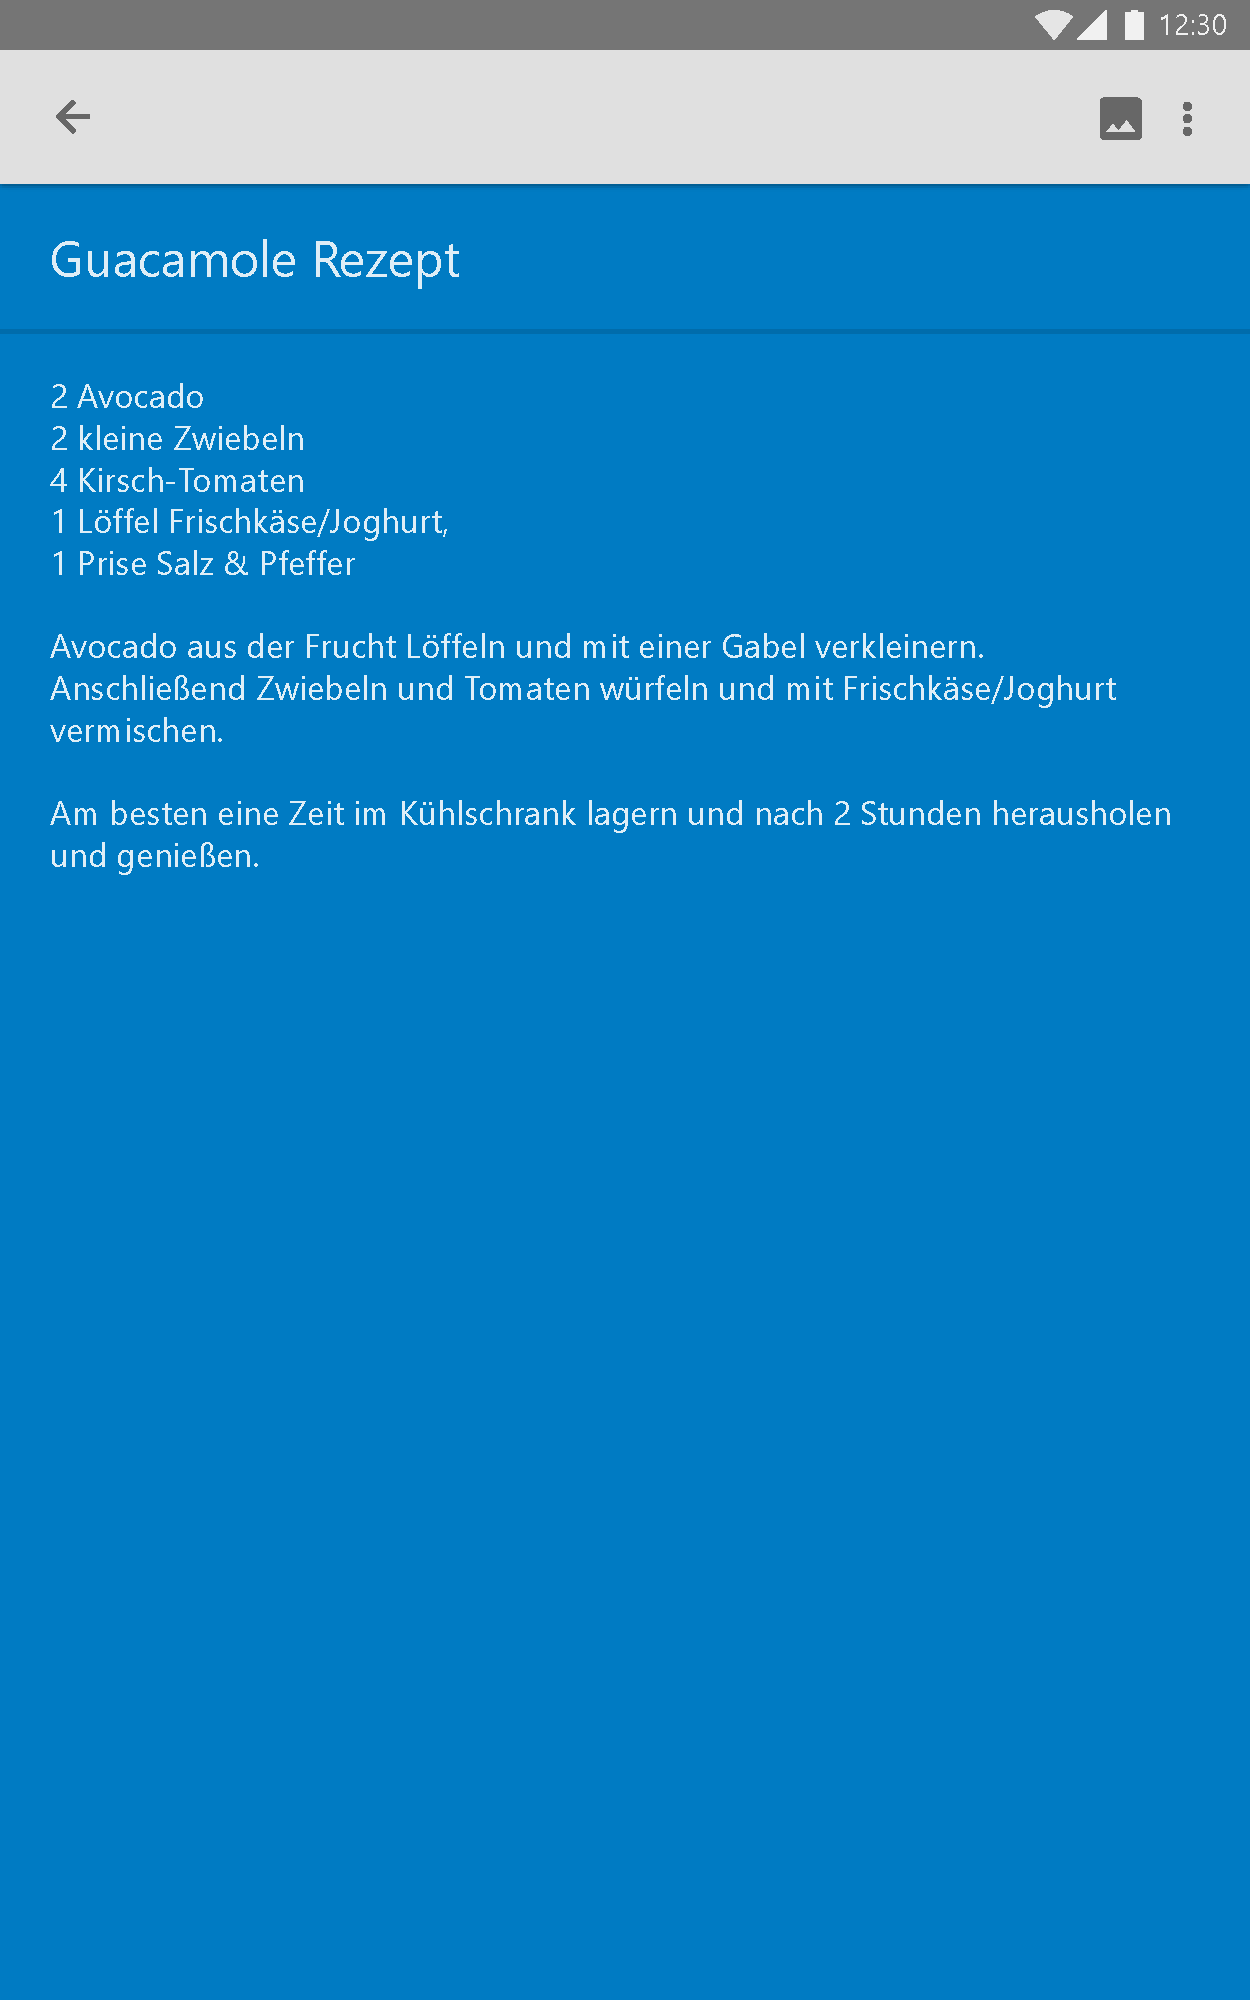
\includegraphics[width=7.25cm]{img/NoteActivity} % Pfad
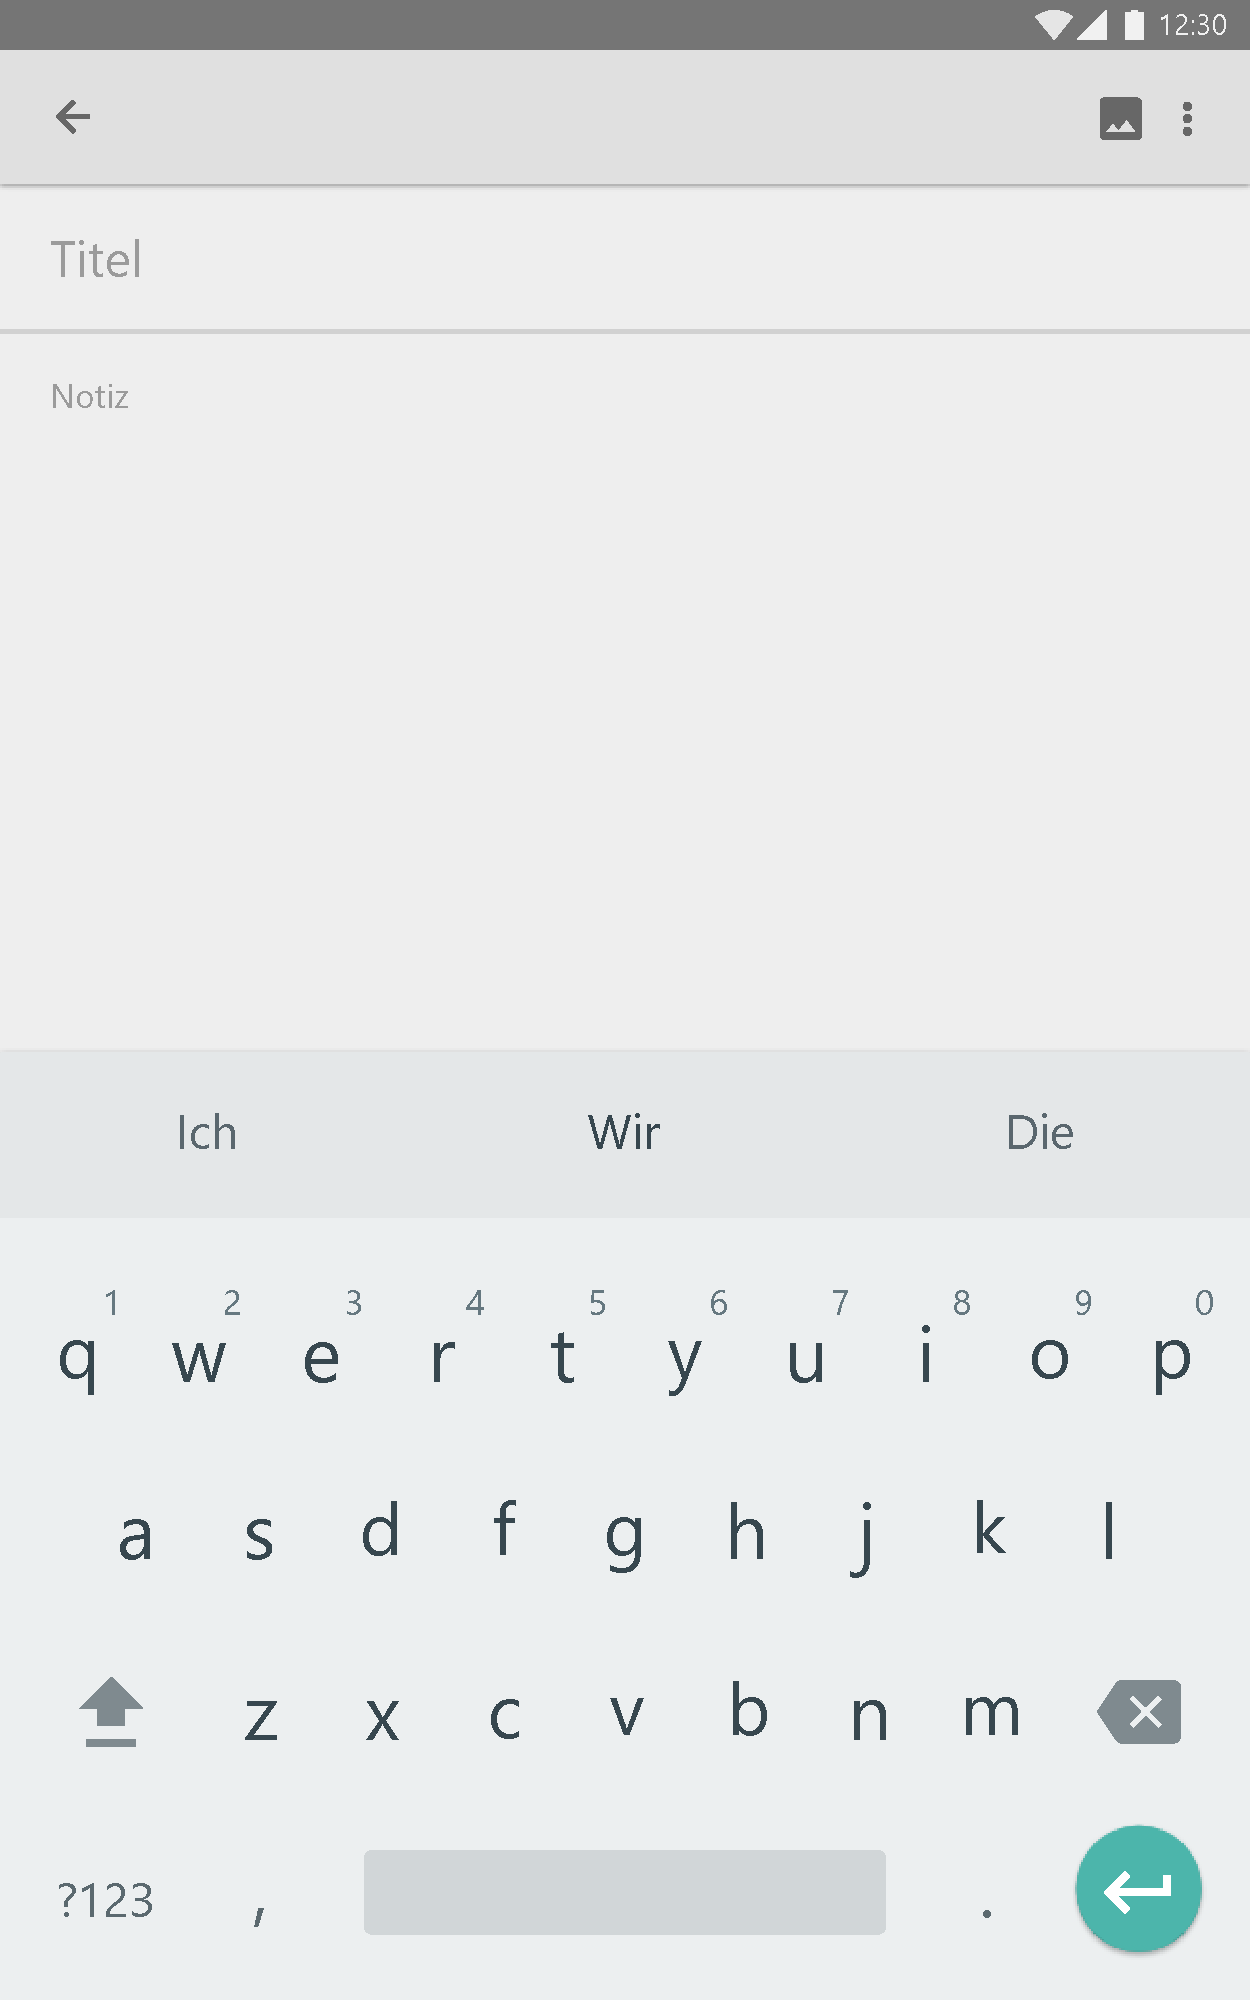
\includegraphics[width=7.25cm]{img/NoteActivityNew}\\ % Pfad
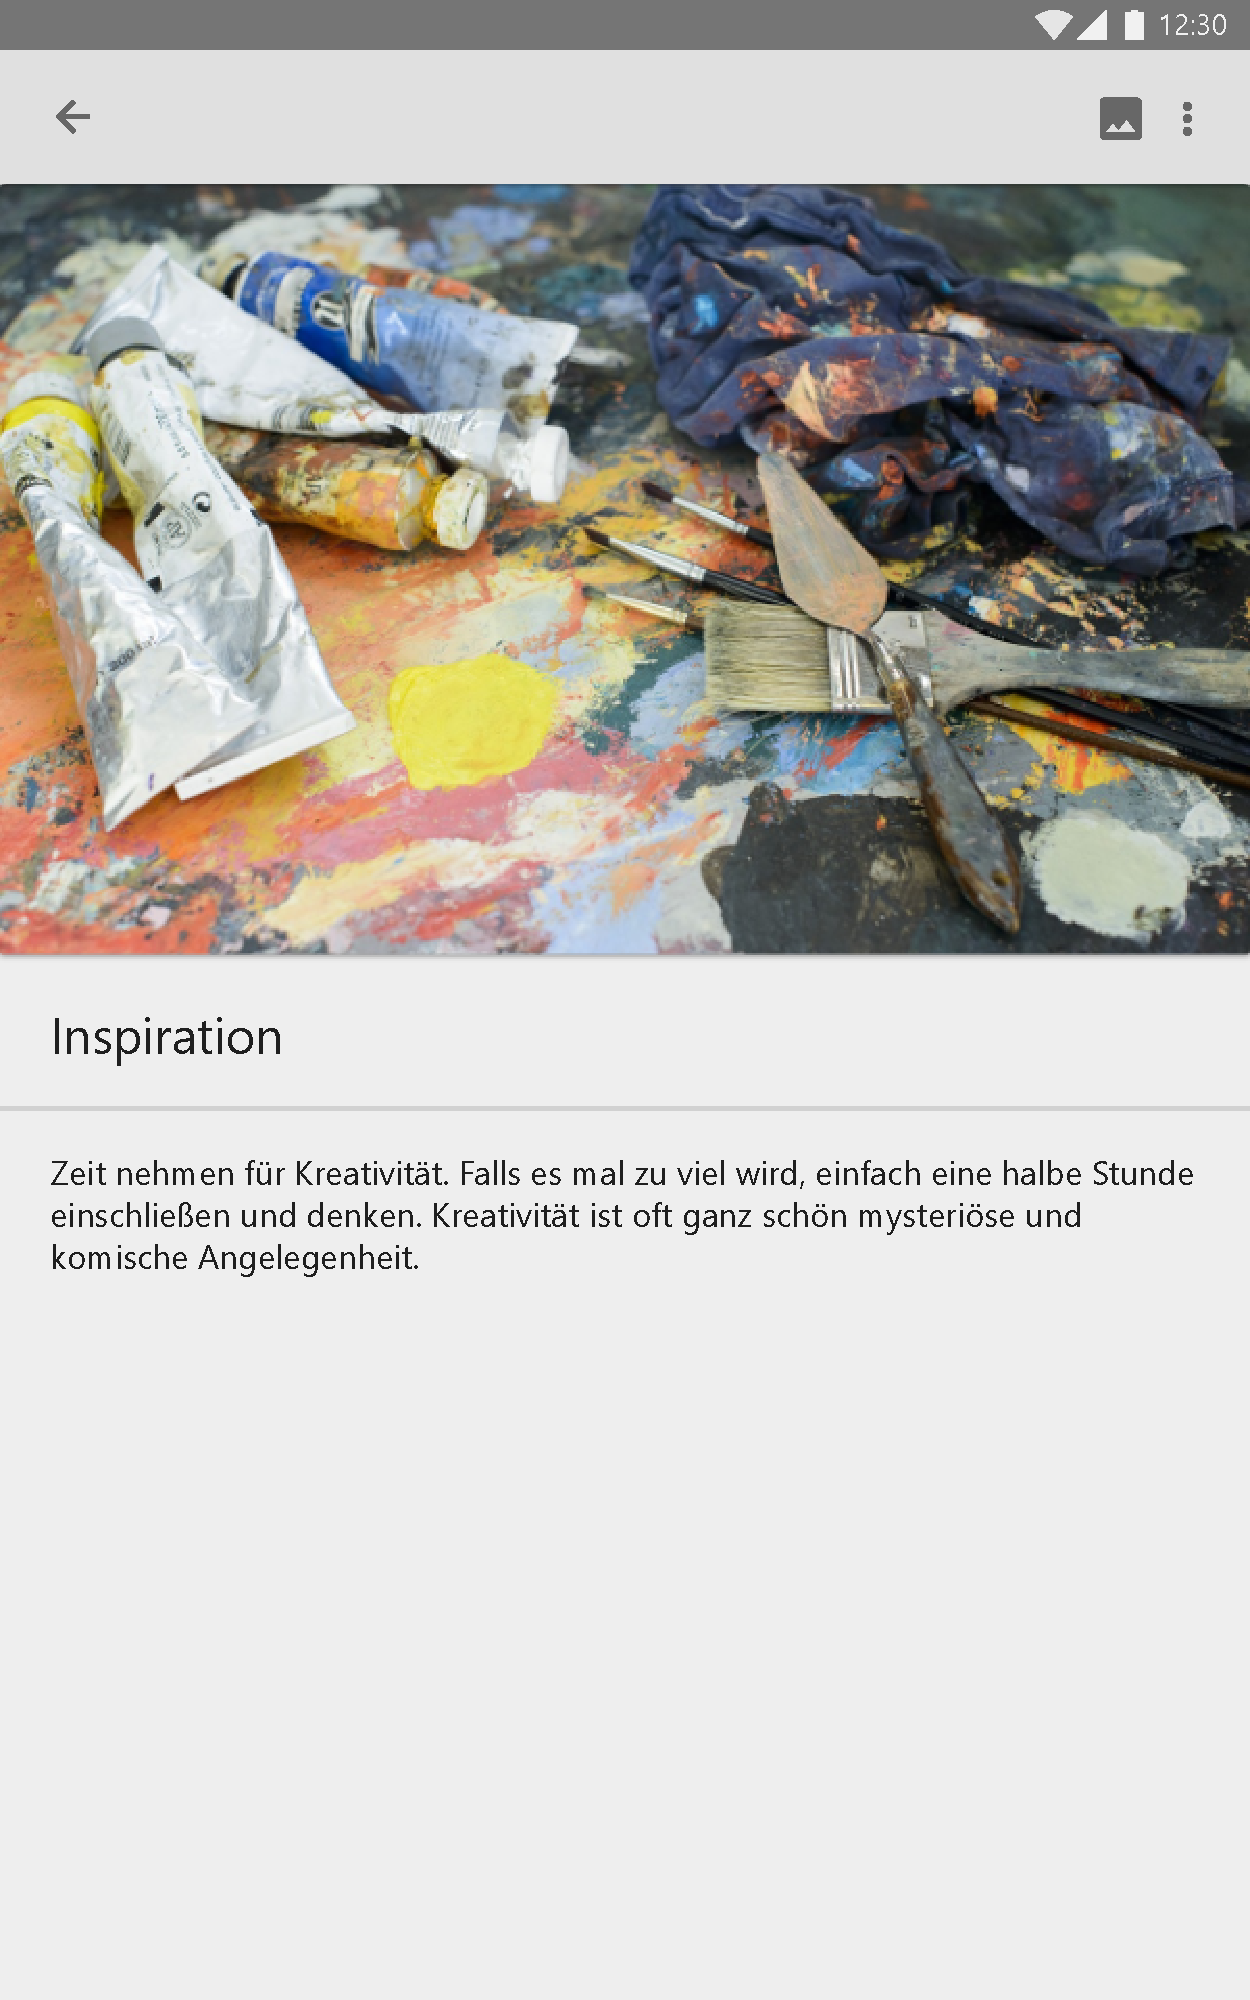
\includegraphics[width=7.25cm]{img/NoteActivityImage}\\ % Pfad
\source{Erstellt von Robin Menzel} % Quelle
\end{minipage}
\end{figure}

\begin{figure}[H]
\centering
\begin{minipage}[t]{1\textwidth} % Breite, z.B. 1\textwidth		
\caption{Mockups - Übersicht über vorhandene und neue Todos} % Überschrift
\includegraphics[width=7.25cm]{img/ToDoActivity} % Pfad
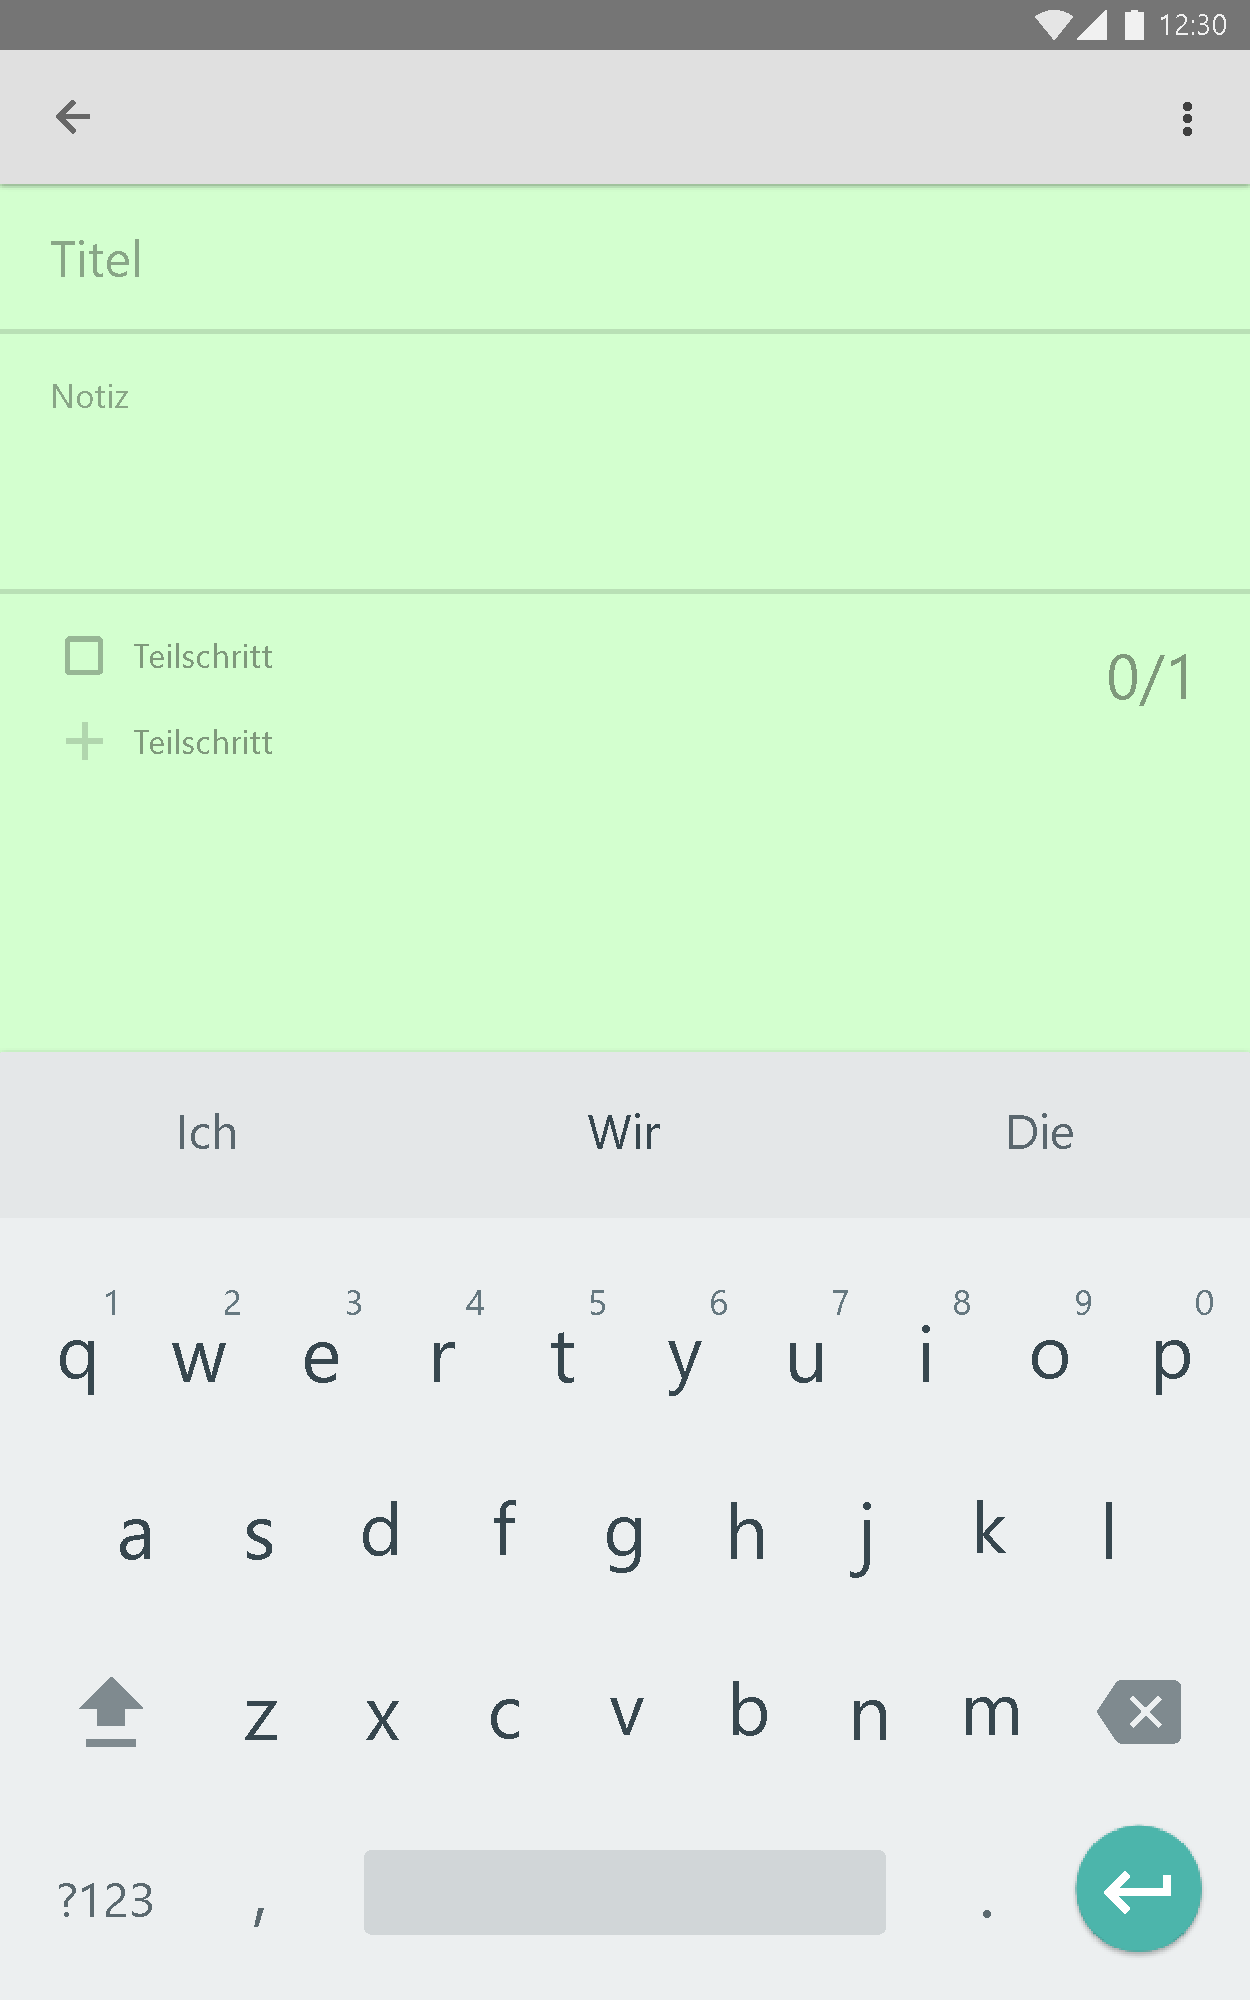
\includegraphics[width=7.25cm]{img/ToDoActivityNew}\\ % Pfad
\source{Erstellt von Robin Menzel} % Quelle
\end{minipage}
\end{figure}

\subsubsection{Planung der Datenstruktur und Schnittstellen (Ruthild Gilles)}
%%%%%%%%%
%Ruthild
%%%%%%%%%

Die gewünschte Applikation soll das Managen von Todos, Events und Notes vereinfachen. Anhand der Anforderungen an die Applikation überlegte sich das Datenteam, welche Daten beziehungsweise Informationen in der Datenstruktur der Applikation abgebildet werden sollen. Da sowohl Todo-, Event-, als auch Note-Objekte einheitlich aufgebaut sein sollen, wurde sich dazu entschieden, dass die jeweiligen Klassen von einer TEN-Klasse erben. Alle Todo-, Event- und Note-Objekte benötigen eine ID zu eindeutigen Identifikation des Objektes auf der Datenbank und in der Applikation. Außerdem könnne die Objekte jeweils einen Titel haben. Zudem sollen die verschiedenen Objekte weitere Informationen enthalten. In folgendem Klassendiagramm sind alle geplanten Attribute der Klassen aufgelistet.

\begin{figure}[H]
\centering
\begin{minipage}[t]{1\textwidth} % Breite, z.B. 1\textwidth		
\caption{Klassendiagramm} % Überschrift
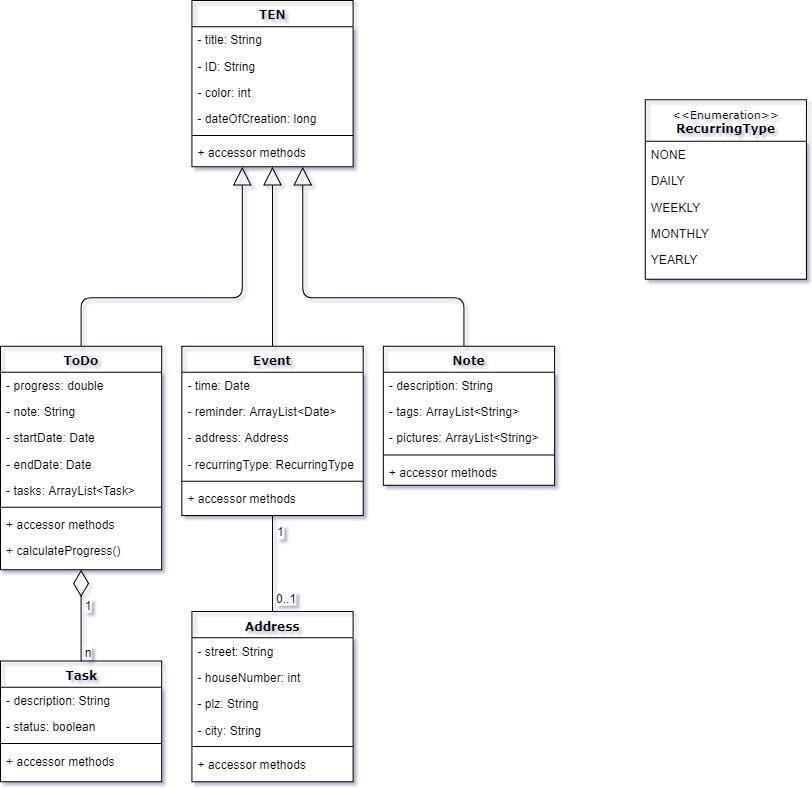
\includegraphics[width=1\textwidth]{img/Klassendiagramm}\\ % Pfad
\source{Erstellt von Joscha Nassenstein} % Quelle
\end{minipage}
\end{figure}

Zusätzlich zu der Struktur der Daten in Form von Klassen mit entsprechenden Attributen wurde ebenfalls die Struktur der Applikation vom Datenteam definiert. Diese ist in nachfolgender Abbildung in einem Systemkontextdiagramm dargestellt.

\begin{figure}[H]
\centering
\begin{minipage}[t]{1\textwidth} % Breite, z.B. 1\textwidth		
\caption{Systemkontextdiagramm} % Überschrift
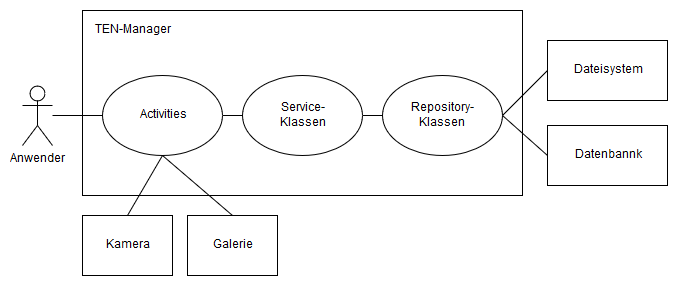
\includegraphics[width=1\textwidth]{img/Systemkontextdiagramm}\\ % Pfad
\source{Erstellt von Ruthild Gilles} % Quelle
\end{minipage}
\end{figure}

Um die Daten auch nach Beendigung der Applikation bei erneutem Starten wieder anzeigen zu können, wurde eine dokumentenbasierte Datenbank an die Applikation angebunden. Auf diese Weise kann eine persistente Datenhaltung erzielt werden. Die einzelnen Activities, welche als Schnittstelle zu den Anwendern dienen, sollen die vom Benutzer eingegebenen Informationen auf der Datenbank speichern können. Dazu sollen Activity-übergreifende Klassen verwendet werden.

Das Datenteam plante die Activity-übergreifenden Klassen und deren Methoden anhand der Anforderungen, der einzelnen Activities. Es sollte möglich sein, einzelne oder auch alle TEN-Objekte von der Datenbank zu erhalten. Auch sollte das Löschen und das Speichern von einzelnen TEN-Objekten möglich sein. Während der Planungsphase wurden hier verschiedene Ansätze in Erwägung gezogen, um diese Anforderungen umzusetzen. Zur Übersichtlichkeit entschied sich das Datenteam letztendlich dafür, einzelne Klassen für jede der vier CRUD-Operationen zu erstellen. Die CRUD-Operationen beinhalten das Erstellen (Create), das Lesen (Read), das Aktualisieren (Update) und das Löschen (Delete) von einzelnen Objekten. Die einzelnen Methoden der CRUD-Klassen sind in folgender Abbildung dargestellt.

\begin{figure}[H]
\centering
\begin{minipage}[t]{1\textwidth} % Breite, z.B. 1\textwidth		
\caption{CRUD-Klassen} % Überschrift
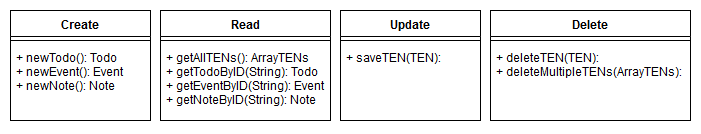
\includegraphics[width=1\textwidth]{img/CRUD-Klassen}\\ % Pfad
\source{Erstellt von Ruthild Gilles} % Quelle
\end{minipage}
\end{figure}

Da der Aufwand für die Umsetzung aller geforderten Anforderungen zu Projektstart lediglich grob geschätzt werden konnte, definierte das Datenteam abgesehen von der Schnittstelle zur Datenbank noch einige weitere Schnittstellen. Die Implementierung dieser weiteren Schnittstellen wurde nicht in den Anforderungen gefordert und würde nur bei genug Zeitüberschuss umgesetzt werden. Zu den weiteren optionalen Schnittstellen gehören das Exportieren von Todos, Events und Notes in die Zwischenablage oder auch in andere Applikationen, die auf dem entsprechenden Endgerät installiert sind. Für ein Event soll es die Möglichkeit geben eine Adresse hinzuzufügen. Hier wäre eine weitere optionale Schnittstelle die Verknüpfung mit Google Maps. Auch könnte eine Schnittstelle zu einer anderen Kalender App implementiert werden, in die ein Event exportiert werden könnte.

\subsubsection{Planung der Activities und Layouts (Florian Rath)}
%%%%%%%%%
%Florian
%%%%%%%%%
In dieser Planungsphase wurde mit einer ausführlichen Anforderungsanalyse begonnen, um die Activities und deren Umfang abschätzen zu können. Der teils unterschiedliche Umfang der Activities ist durch die gegebenen Anforderungen zustande gekommen.

Außerdem wurde geprüft ob die Activities Beziehungen aufweisen. Als Activities wurden zuerst das Todo, Event und Note (TEN) identifiziert. Die gesamte Darstellung der TENs sollte in einer Übersicht erfolgen, der Overview. Die Overview bildet eine weitere wichtige Activity, um der App eine übersichtliche Darstellung zu geben.
 
Nach der Anforderungsanalyse wurden die Activities in Aufgabenpakete zerlegt, um diese auf die Teammitglieder verteilen zu können. Die Layouts können diesen Activities zugewiesen werden und sind daher logisch an diese gebunden. Der Aufbau der Layouts soll sich an dem erstelltem MockUp orientieren, um der App einen einheitlichen und ansehnlichen Look zu verpassen.

Nachdem die Planung für die Aufteilung der Activities feststand, wurde diese mit den Teammitglieder abgesprochen. 

\subsubsection{Planung der Navigation zwischen den Activities (Yannick Rüttgers)}
%%%%%%%%%
%Yannick
%%%%%%%%%

Als Einstiegspunkt für den Nutzer soll eine Übersichtsactivity dienen. Von dieser aus sollen alle weiteren Activities aufgerufen werden können.

Die einzelnen Activities sollen auf zwei Arten aufgerufen werden können. Entweder soll ein neues TEN erstellt werden, oder ein bereits vorhandenes angezeigt werden.

Wenn ein neues TEN erstellt werden soll, soll die zugehörige Activity ohne weitere Parameter aufgerufen werden. Dadurch soll in dieser dann ein leeres TEN erstellt werden, welches dann bearbeitet werden kann.

Soll stattdessen ein bereits bestehendes TEN angezeigt werden, wird der Activity die ID des jeweiligen TEN übergeben, welches dann im weiteren Verlauf von der Activity geladen und angezeigt wird.

Wird aus den jeweiligen TEN-Activities zurücknavigiert, soll wieder die Übersichtsactivity angezeigt werden, in der die getätigten Änderungen angezeigt werden sollten.

\newpage
\subsection{Geplante Aufgabenverteilung im Team (Fabia Schmid)}
%%%%%%%%%
%Fabia
%%%%%%%%%

\begin{longtable}{|p{4cm}|p{10cm}|}
\hline
{\textbf{Name}} & {\textbf{Aufgaben}}  \\ \hline
Ruthild Gilles & Erstellung Service-Klassen,

Schreiben eines Protokolls,

Projekttagebuch führen, 

Dokumentation anfertigen \\ \hline 
Fabia Schmid  & Projektsteuerung und -planung, 

Erstellung der Layouts für die ActivityOverview,  

Erstellung der OnClickListener für die ActivityOverview,  

Projekttagebuch führen, 

Dokumentation anfertigen \\ \hline

Jan Beilfuß & Einbindung der Datenbank, 

Erstellung der Event Activity,

Projekttagebuch führen, 

Dokumentation anfertigen \\ \hline
Yannick Rüttgers & Erstellung ActivityOverview,  

Planung der Navigation zwischen Klassen, 

Erster Latexentwurfprojekttagebuch, 

Latex-Beauftragter, 

Projekttagebuch führen, 

Dokumentation anfertigen \\ \hline
Robin Menzel & Zusammenführung des Quellcodes, 

Erstellung des Mockups, 

Erstellung der Event Activity, 

Projekttagebuch führen, 

Dokumentation anfertigen \\ \hline
Florian Rath  & Aufteilung der Activities, 

Erstellung Activity ToDo, 

Projekttagebuch führen, 

Dokumentation anfertigen \\ \hline
Joscha Nassenstein & Erstellung von Note, 

Erstellung der TEN-Klassen,  

Erstellung Datendiagramm, 

Projekttagebuch führen, 

Dokumentation anfertigen \\ \hline
Sertan Cetin &  Aufteilung der Activities, 

Erstellung Activity ToDo, 

Projekttagebuch führen, 

Dokumentation anfertigen \\ \hline
\end{longtable}

